\documentclass[problems]{esg8012pset} 
  \usepackage{amsmath}
  \usepackage{amssymb}
  \usepackage{enumerate}
  \usepackage{graphicx}
  \usepackage{hyperref}
  %\usepackage{siunitx}
  \providecommand{\uvec}[1]{{\hat{\bf{#1}}}}
  \usepackage{pgf,tikz}
  \usetikzlibrary{arrows}
  \makeatletter
  \newcommand{\interitemtext}[1]{%
    \begin{list}{}
     {\itemindent=0mm\labelsep=0mm
     \labelwidth=0mm\leftmargin=0mm
     \addtolength{\leftmargin}{-\@totalleftmargin}}
      \item #1
    \end{list}
  }
  \makeatother
  \renewcommand{\d}{\,d}
  \providecommand{\norm}[1]{\lVert#1\rVert}
\classname{Physics 8.012} 
\semester{Fall 2010} 
\problemsetnumber{6} 
\date{October 15} 
\duedate{Monday, October 25} 
\readingassignment{Kleppner and Kolenkow, \emph {An Introduction to Mechanics}, Chapter Four} 
\begin{document}
\section{Problem \thesection: K\&K 4.2}
  A block of mass $m$ slides along a horizontal table with speed $v_0$. At $x = 0$ it hits a spring with spring constant $k$ and begins to experience a friction force. The coefficient of friction is variable and is given by $u_k = bx$, where $b$ is a constant. What is the change in mechanical energy when the block has first come momentarily to rest?
  \begin{center}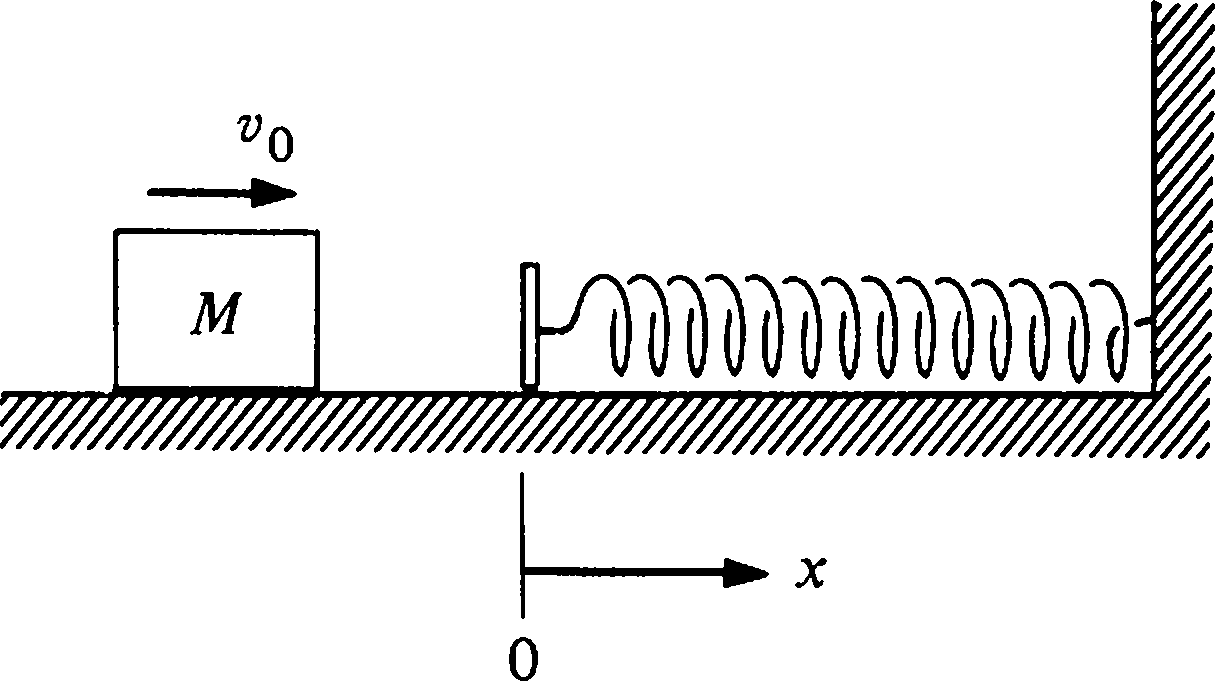
\includegraphics[width=0.4\textwidth]{ps06_1}\end{center}
\section{Problem \thesection: K\&K 4.5}
  A body of mass $m$ whirls around on a string which passes through a fixed ring located at the center of the circular motion. The string is held by a person who pulls the string downward with a constant velocity of magnitude $V$ so that the radial distance to the body decreases from an initial distance $r_0$ to a final distance $r_f$ from the center. The body has an initial angular velocity $\omega_0$. You may neglect the effect of gravity. Show that the work done in pulling the string equals the increase in kinetic energy of the body.
\section{Problem \thesection: K\&K 4.7}
  A ring of mass $m_r$ hangs from a thread, and two identical beads of mass $m_b$ slide on it without friction. The beads are released simultaneously from the top of the ring and slide down opposite sides.
  \begin{center}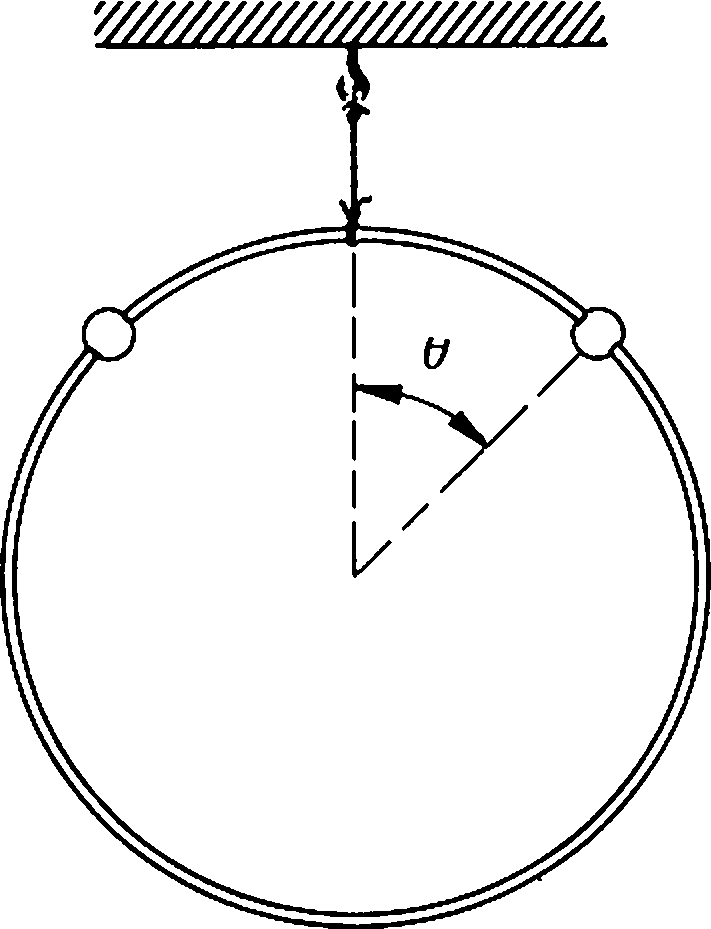
\includegraphics[width=0.2\textwidth]{ps06_2}\end{center}
  \begin{enumerate}[(a)]
    \item Draw free body force diagrams for the ring and the beads. What direction is the force of the bead on the ring pointing? Does it change has the bead moves. Can you still proceed with an analysis using Newton's Second Law if you are not sure which way this force points? Try to find a physical explanation for the direction of this force.
    \item Show that the ring will start to rise if $m_b > (3/2)m_r$, and find the angle $\theta$ with respect to the vertical direction that this occurs.
  \end{enumerate}
\section{Problem \thesection: K\&K 4.9}
  Consider the exothermic reaction (final kinetic energy is greater than the initial kinetic energy).
  $$\text{H} + \text{H} \to \text{H}_2 + 5\text{ eV}$$
  Two hydrogen atoms collide and produce a diatomic hydrogen molecule. However, when hydrogen atoms collide in free space they simply bounce apart. The reason is that it is impossible to satisfy the laws of conservation of energy and momentum in a simple two body collision which releases energy.
  \begin{enumerate}[(a)]
  \item Can you prove this? Try to analyze this collision in a reference frame moving with the velocity of the center of mass of the system.
    \item Can this two body reaction take place if the temperature is dramatically lowered to near zero degrees Kelvin? Try to give an physical explanation for your answer.
  \end{enumerate}
\section{Problem \thesection: K\&K 4.10}
  A block of mass $m_b$ on a horizontal table is connected to one end of a spring with spring constant $k$. The other end of the spring is attached to a wall. The block is set in motion so that it oscillates about its equilibrium point with amplitude $A_0$.
  \begin{enumerate}[(a)]
  \item What is the period of the motion?
    \interitemtext{A lump of sticky putty of mass $m_p$ is dropped onto the block. The putty sticks without bouncing. The putty hits the block at the instant when the velocity of the block is zero.}
    \item Find the new period, the new amplitude, and the change in mechanical energy of the system.
    \interitemtext{The putty is removed and the block is set in motion. This time the putty is dropped and hits the block at the instant the block has its maximum velocity.}
    \item Find the new period, the new amplitude, and the change in mechanical energy of the system.
  \end{enumerate}
\section{Problem \thesection: K\&K 4.12}
  During the Second World War the Russians, lacking sufficient parachutes for airborne operations, occasionally dropped soldiers inside bales of hay onto snow. The human body can survive an average pressure of 30 lbs / in$^2$. Suppose that the lead plane drops a dummy bale equal in weight to a loaded one from an altitude of 150 ft, and that the pilot observes that it sinks about 2 ft into the snow. If the weight of an average soldier is 144 lbs and his effective area is 5 ft$^2$, is it safe to drop the men?
\section{Problem \thesection: K\&K 4.13}
  A commonly used potential energy function to describe the interaction between two atoms is the Lennard-Jones 6,12 potential
  $$U(r) = \varepsilon\left[(r_0 / r)^{12} - 2(r_0 / r)^6\right].$$
  \begin{enumerate}[(a)]
  \item Show that the radius at the potential minimum is $r_0$, and that the depth of the potential well is $\varepsilon$.
    \item Find the angular frequency of small oscillations about the stable equilibrium position for two identical atoms of mass $m$ bound to each other by the Lennard-Jones interaction.
  \end{enumerate}
\end{document}
